\lecture{26}{2025-05-21}{Examen final approche}{}


\begin{parag}{Application: changement de variable polaire}
    \begin{align*} \psi \left(r, \phi\right) =  
        \begin{cases}
            x =  r \cos \phi\\
            y =  r \sin \phi
        \end{cases} \mathspace \mathspace \psi : \mathbb{R}_+ \times [ 0, 2\pi [ \to \mathbb{R}^{2} \setminus \left\{0\right\}
    \end{align*}
    avec $\psi$ qui est bijective\\
        On a donc pour la jacobienne:
        \begin{align*}
            J_{\phi}\left(r, \phi\right) =  \begin{pmatrix} \cos \phi & -r\sin \phi \\ \sin\phi & r\cos\phi \end{pmatrix}  \implies \det J_{\psi \left(r, \phi\right)} =  r \left(\cos^2\phi + \sin^2\phi\right) =  r
        \end{align*}

    \begin{center}
        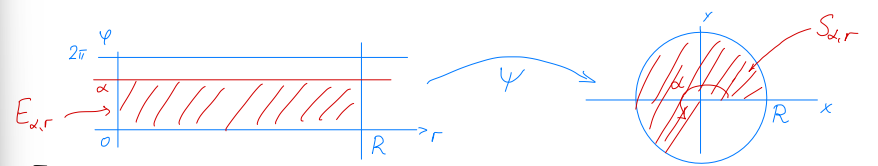
\includegraphics[scale=0.7]{12025-05-21.png}
    \end{center}
\end{parag}
\begin{parag}{Exemple 1}
    On cherche l'aire du secteur circluaire $S_{\alpha, r}$ d'angle $\alpha$ et de rayon $R$:
    \begin{center}
        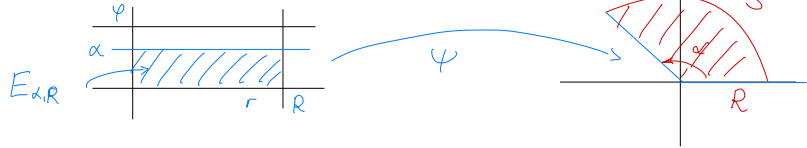
\includegraphics[scale=0-7]{22025-05-21.png}
    \end{center}
    On a donc:
    \begin{align*} A_{\alpha, r} =  \int\int_S 1 dxdy =  \int_0^\alpha d\phi \int_0^R \left| \det \psi_{r, \phi}\right|dr\\
        = \int_0^\alpha d\phi \int_0^R r dr =  \alpha \frac{1}{2} r^2\mid_0^R =  \frac{1}{2}R^2 \alpha
    \end{align*}
    Si $\alpha = 2\pi \implies $ l'aire du disque du rayon $R$ est:
    \begin{align*} A_{2\pi, R} =  \frac{1}{2} R^2 \cdot  2\pi =  \pi R^2 \end{align*}
    
\end{parag}
\begin{parag}{Exercice}
    L'aire du disque de rayon $1$ en coordonnées cartesiennes.
    \begin{align*} D =  \left\{\left(x, y\right) \in \mathbb{R}^{2}: x^2 + y^2 \leq 1\right\} \end{align*}
    On a donc l'intégrale qui est donnée par:
    \begin{align*} 
        A =  \int_{-1}^1 dx \int_{-\sqrt{1 - x^2}}^{\sqrt{1 - x^2}}1 dy =  \int_{-1}^1 2 \sqrt{1 - x^2}dx
    \end{align*}
    Ensuite on peut poser le changement de variable $x \sin t$. On utilisera aussi le fait que notre fonction est paire afin de calculer ``qu'une seule fois'' l'intégrale comme ceci:
    \begin{align*} 4 \int_0^2 \sqrt{1-x^2}dx \end{align*}
\end{parag}

\subsubsection{Conclusion: changement de variable polaires}


\begin{parag}{Cas important: Coordonnées polaires}
    \begin{align*} G \left( r, \phi\right) =  
        \begin{cases}
            r  \cos \phi =  x\\
            r \sin \phi =  y
        \end{cases}
    \end{align*}
    \begin{center}
        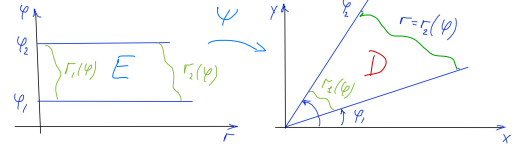
\includegraphics[scale=0.8]{32025-05-21.png}
    \end{center}
\end{parag}
\begin{parag}{Exemple}
    soit $f\left(x, y\right) = \sqrt{a^2 - x^2 - y^2}$ avec $a > 0$, $D$ est une boucle de lemmiscate de Bernouilli (1694):
    \begin{align*} \left(x^2 + y^2\right)^2 =  a^2\left(x^2 - y^2\right) \;\; x > 0 \end{align*}
    Si on chercher maintenant à le placer en coordonnées polaires:
    \begin{align*} 
        r^4 =  a^2\left(r^2\cos^2\phi - r^2 \sin^2 \phi\right) =  a^2 r^2 \cos 2\phi\\
        \iff r^2 =  a^2 \cos 2 \phi \implies \cos 2 \phi \geq 0
    \end{align*}
    Et donc:
    \begin{align*} 
        \cos 2 \phi > 0 \implies - \frac{\pi}{2} < 2\phi < \frac{\pi}{2} \\
        \implies - \frac{\pi}{4} \leq \phi \leq \frac{\pi}{4} \\
        \frac{3\pi}{4}< \phi < \frac{5\pi}{4} \; \; x <0
    \end{align*}
    On a donc finalement:
    $r =  a \sqrt{\cos 2 \phi}$ avec $- \frac{\pi}{4} \leq \phi \leq \frac{\pi}{4}$ qui est l'équation d'une boucle de la lemmiscate. \\
    Si on prends les deux ``maximum'', $\phi = \pm \frac{\pi}{4} \implies r = 0$ et ensuite $\phi =  0 \implies r = a$, on a donc finalement pour l'ensemble:
    \begin{align*} 
        E =  \left\{-\frac{\pi}{4} < \phi < \frac{\pi}{4}, 0 < r < a\sqrt{\cos 2 \phi} \right\}
    \end{align*}
        \begin{center}
            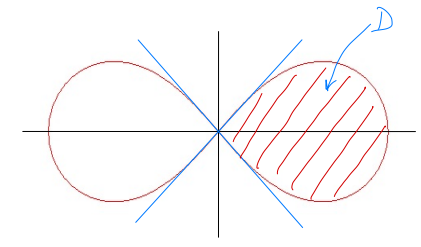
\includegraphics[scale=0-8]{42025-05-21.png}
        \end{center}
        On a donc avec un changement de variable:
        \begin{align*} 
            \int\int_D \sqrt{a^2 - x^2 - y^2} dxdy &= \int\int_E \sqrt{a^2-r^2} \underbrace{r}_{\left|\det J\right|}dr d\phi\\
            \int_{-\frac{\pi}{4}}^{\frac{\pi}{4}}d\phi \int_0^{a\sqrt{\cos 2\phi}}\sqrt{a^2 - r^2} rdr
        \end{align*}
        On voit ici qu'on peut juste faire un changement de variable $u = a^2 - r^2$ ce qui au vu du $r$ qui ``depasse'' de la racine va se simplifier:
        \begin{align*} 
            -\frac{1}{2}\int_0^{a\sqrt{\cos 2\phi}}\sqrt{a^2 - r^2}d\left(a^2 - r^2\right)\\ 
            &=  -\frac{1}{2} \cdot  \frac{2}{3} \left(a^2 - r^2\right)^{\frac{3}{2}}\mid_{0}^{a\sqrt{\cos 2\phi}}\\ 
            &= - \frac{1}{3}\left(a^2 - a^2 \cos 2 \phi\right)^{\frac{3}{2}} + \frac{1}{3}a^3
        \end{align*}
        Donc si on essaie de simplifier  tout ça:
        \begin{align*} 
            \left(1-\cos 2 \phi\right)^{\frac{3}{2}} =  \left(-\cos^2\phi + \sin^2\phi\right)^{\frac{3}{2}} = 2^{\frac{3}{2}}\left(\sin^2\phi\right)^{\frac{3}{2}} =  2^{\frac{3}{2}}\left|\sin\phi\right|^{3}
        \end{align*}
        Et donc on peut intégrer:
        \begin{align*} 
            \int_{-\frac{\pi}{4}}^{\frac{\pi}{4}} \left( - \frac{1}{3} 2^{\frac{3}{2}}a^3 \left|\sin \phi\right|^3 + \frac{1}{3}a^3\right) d\phi\\
            &=  \frac{1}{3}a^3 \left(\frac{\pi}{4} + \frac{\pi}{4}\right) - \frac{1}{3}a^3 2^{\frac{3}{2}}\int_{-\frac{\pi}{4}}^{\frac{\pi}{4}}\left| \sin\phi\right|^3 d\pih \\
            &= \frac{\pi}{6}a^3 - \frac{1}{3}a^3 2^{\frac{3}{2}}\cdot 2 \int_0^{\frac{\pi}{4}} \sin^3 \phi d \phi
        \end{align*}
        \begin{align*} 
            \int_0^{\frac{\pi}{4}} \sin^3 \phi d\phi &=  \int_0^{\frac{\pi}{4}}\left(-1 \cos^2\phi\right)d\left(-\cos\phi\right) \\
                                                     &=  \frac{1}{3} \cos^3\phi - \cos\phi \mid_0^{\frac{\pi}{4}} \\
                                                     &=  \frac{1}{3}\left(\frac{1}{\sqrt{2}}\right)^3 - \frac{1}{\sqrt{2}} - \frac{1}{3} + 1\\
            \frac{2}{3} + \frac{1}{\sqrt{2}}\left(\frac{1}{6} - 1\right) &=  \frac{2}{3}  - \frac{5}{6\sqrt{2}}
        \end{align*}
        Et donc si on remet tout ça dans notre intégrale en haut (qui comment par $\frac{\pi}{6}$)
        \begin{align*} 
            \int\int =  \frac{\pi a^3}{6} - \frac{a^3 \cdot  2^{\frac{3}{2}} \cdot  2}{3} \left(\frac{2}{3} - \frac{5}{6\sqrt{2}}\right) 
        \end{align*}
\end{parag}

\begin{parag}{Exemple 3}
    Soit $f\left(x, y\right) =  xy$ avec $D =  \left\{ \left(x + 1\right)^2 + y^2 \leq 1 , y \geq \frac{x}{\sqrt{3}}\right\}$\\
On voit en premier lieu que notre ensemble à une condition qui ressemble à un disque donc on peut essayer d'utiliser un changement de variable:
\begin{align*} 
    r^2\cos^2\phi + 2r\cos\phi + 1 + r^2\sin^2\phi \leq 1 &\implies r^2 + 2r\cos\phi \leq 0\\
    t + 2\cos\phi \leq 0 &\implies r \leq -2\cos\phi \implies \cos\phi < 0\\
                         &\implies \frac{\pi}{2} < \phi < \frac{3\pi}{2}
\end{align*}
Si on prends maintenant la deuxième condition avec un changement de variable polaire:
\begin{align*} 
    y \geq \frac{x}{\sqrt{3}} &\implies r \sin \phi \geq \frac{r \cos \phi}{\sqrt{3}}\\
                              &\implies \sin\phi \geq \frac{\cos \phi}{\sqrt{3}}\\
\end{align*}
Ce qui nous donne deux cas, soit $\sin\phi > 0, \cos \phi < 0 \implies \frac{\pi}{2} < \phi < \pi$. ou alors $\sin \phi < 0, \cos\phi < 0 \implies \tan \phi < \frac{1}{\sqrt{3}}$.\\
et donc si on développe pour $\phi$ on a:
\begin{align*} 
    \tan \phi =  \frac{1}{\sqrt{3}} \implies \phi =  \frac{\pi}{6} + \pi k \implies \pi < \phi < \frac{7}{6}\pi
\end{align*}
On a donc notre ensemble qui est:
\begin{align*} 
    E =  \left\{\frac{\pi}{2} < \phi < \frac{7}{6}\pi, 0 < r < -2 \cos\phi\right\}
\end{align*}
Il reste plus qu'a intégrer:
\begin{align*} 
    \int\int_D xy dxdy &=  \int_{\frac{\pi}{2}}^{\frac{7\pi}{6}}d\phi \int_0^{-2\cos\phi}r^2 \cos\phi s\sin\phi r dr\\
                       &= \int_{\frac{\pi}{2}}^{\frac{7\pi}{6}}d\phi \left(\frac{1}{4}r^4 \cos \phi \sin\phi\right)\mid_0^{-2\cos\phi}\\
                       &= 4 \int_{\frac{\pi}{2}}^{\frac{7\pi}{6}}\cos^5\phi\sin\phi d\phi\\
                       &= -4 \int_{\frac{\pi}{2}}^{\frac{7\pi}{6}}\cos^5\phi d \cos \phi\\ 
                       &= - \frac{4}{6}\cos^6 \phi \mid_{\frac{\pi}{2}}^{\frac{7\pi}{6}} =  \cos \frac{7\pi}{6} =  -\cos \frac{\pi}{6} =  -\frac{\sqrt{3}}{2}
\end{align*}
\begin{center}
    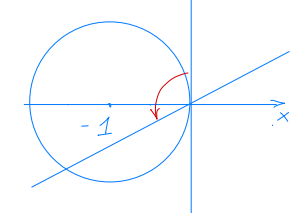
\includegraphics[]{52025-05-21.png}
\end{center}
\begin{subparag}{Coordonnées cartesiennes}
    \begin{align*} 
        D =  \left\{\left(x + y\right)^2  + y^2 \leq 1, y \geq \frac{x}{\sqrt{3}} \right\}
    \end{align*}
    On a donc:
    \begin{align*} 
        y =  \frac{x}{\sqrt{3}} \implies \left(x + 1\right)^2 + \frac{x^2}{3} =  1 \\
        \implies \frac{4}{3}x^2 + 2x + 1 =  1 = \begin{cases} x =  0 \\ \frac{4}{3}x =  -2 \end{cases}
    \end{align*}
    Ce qui implique donc que:
    \begin{align*} 
         \begin{cases}
             x =  0\\ x = -\frac{2}{3}
         \end{cases} , \; y =  - \frac{\sqrt{3}}{2}
    \end{align*}
    On a donc pour l'autre condition:
    \begin{align*} 
        y^2 \leq 1 - \left(x + 1\right)^2 \implies -\sqrt{1 - \left(x + 1\right)^2} <y< \sqrt{1 - \left(x + 1\right)^2}
    \end{align*}
    Et cela sur $D_1$.
    \begin{align*} 
        \frac{x}{\sqrt{3}} < y < \sqrt{1 - \left(x + 1\right)^2}
    \end{align*}
    Si on met donc l'union de nos deux ensemble ensemble:

    \begin{align*} 
    D =  \left\{-2 \leq x \leq -\frac{3}{2}, - \sqrt{1 - \left(x + 1\right)^2} < y < \sqrt{1 - \left(x + 1\right)^2}\right\}\\
    \bigcap \left\{\frac{-3}{2}<x<0, \frac{x}{\sqrt{3}} < y < \sqrt{1 - \left(x + 1\right)^2}\right\}
    \end{align*}
    On peut ensuite intégrer sur cette ensemble.
\end{subparag}
\end{parag}

\subsubsection{Coordonnées sphérique}
\begin{parag}{Coordonnée sphérique}
    \begin{align*} 
        G \left( r, \theta, \phi\right) = \begin{cases} x =  r \sin\theta \cos\phi\\ y =  r\sin\phi \sin \theta\\ z = r\cos\theta\end{cases}
    \end{align*}
    On a  donc $G:  ] 0, \infty [ \times [ 0, \pi ] \times [ 0, 2\pi [ \to \mathbb{R}^{3}\setminus \left\{\overline{0}\right\} $\\
    On peut donc calculer la jacobienne qui est donné par:
    \begin{align*} 
        J_{G\left(r, \theta, \phi\right)} = \begin{pmatrix} \sin \theta\cos\phi & r\cos\theta\cos\phi & -r\sin\theta\cos\phi \\ \sin\theta\sin\phi & r\cos\theta\sin\phi & r\sin\theta\cos\phi \\ \cos\theta & -r\sin\theta & 0 \end{pmatrix} 
    \end{align*}
    Je passe les calculs avec la règle de Sarrus mais  on obtient:
    \begin{align*} 
        \left|\det J_{G\left(r, \theta, \phi\right)}\right| =  \left|r^2\cos^2\theta\sin\theta + r^2\sin^3\theta\right| =  \left|r^2\sin\theta\right| \mathspace 0 < \theta < \pi
    \end{align*}

\end{parag}


\begin{parag}{Exemple, Volume d'une boule de rayon $a > 0$}
    On a donc pour l'ensemble:
    \begin{align*} 
        E =  \left\{0 < r < a, 0 < \theta < \pi, 0 < \phi < 2\pi\right\}
    \end{align*}
    On a donc pour le volume:

    \begin{align*} 
        V &=  \int\int\int_{B\left(\overline{0}, a\right)} 1 dxdydz &= \int_0^{2\pi}d\phi\int_0^\pid\theta\int_0^a r^2\sin\theta dr\\
          &= \int_0^{2\pi}d\phi\int_0^\pi\sin\theta d\theta \cdot  \int_0^a r^2 dr\\
          &= 2\pi\left(-\cos\theta\right)\mid_0^\pi \cdot  \frac{1}{3}r^3 \mid_0^a \\
          &= 2\pi\left(1 + 1\right) \cdot  \frac{1}{3}a^3 =  \frac{4}{3}\pi a^3 
    \end{align*}
\end{parag}

\subsubsection{Application: masse totale d'un objet solide}
\begin{parag}{Masse total d'un objet de solide de densité donnée}
    \begin{align*} 
        M = \int\int\int_V \rho \left(x, y, z\right) dxdydz
    \end{align*}
    est la masse totale du volume $V$ avec la densité $\rho\left(x,y, z\right)$
\end{parag}
\begin{parag}{Exemple}
    Trouver la masse totale d'un secteur sphérique:
    \begin{align*} 
        S = \left\{x > 0, y > 0, z > 0, x^2 + y^2 + z^2 < a^2\right\}
    \end{align*}
    Avec la fonction de densité $\rho \left(x, y, z\right) =  x^2 + y^2$.\\
    On a va donc comme on l'a fait juste avant, effectuer une changement de variable en coordonnées sphérique ce qui nous donne donc:
    \begin{align*} 
        E =  \left\{0 < r < a, 0 < \theta < \frac{\pi}{2}, 0 < \phi < \frac{\pi}{2}\right\}
    \end{align*}
    Ce qui nous donne donc:
    \begin{align*} 
        M &=  \int\int\int_S \left(x^2 + y^2\right) dxdydz = \int_0^{\frac{\pi}{2}}d\ph\iint_0^{\frac{\pi}{2}}d\theta \int_0^a r^2 \sin^2 \theta \underbrace{r^2 \sin \theta}_{\left|\det J\right|}dr\\
         &=  \int_0^{\frac{\pi}{2}} d\phi \int_0^{\frac{\pi}{2}}\sin^3\theta d \theta \int_0â r^4 dr\\
         &= \frac{\pi}{2}\int_0^{\frac{\pi}{2}}\left(\cos^2\theta - 1\right)d\cos \theta \cdot \frac{1}{5}r^5\mid_0^a = \frac{\pi}{2}\left(\frac{1}{3}\cos^3\theta - \cos \theta\right)\mid_0^{\frac{\pi}{2}} \cdot  \frac{1}{5}a^5\\
         &= \frac{\pi a^5}{10}\left(-\frac{1}{3} + 1\right) =  \frac{\pi a^5}{15}
    \end{align*}

\end{parag}
\begin{parag}{Question du jour}
    \begin{align*} f\left(x, y\right) =  2x + 3y \end{align*}
    Avec
    \begin{align*} D = \left\{\left(x, y\right) \in \mathbb{R}^{2}: x < 0, y > 0, 1 < x^2 + y^2 < 4\right\} \end{align*}
    Alors $\int\int_D f\left(x, y\right) dxdy $ vaut?\\
    Alors en premier lieu on peut changer en coordonnée polaire:
    \begin{align*} 
        D = \left\{\left(r, \phi\right): r \cos \phi < 0, r \sin \phi > 0, 1 < r^2 < 4\right\}
    \end{align*}
    On écrit notre fonction en coordonnée
    \begin{align*} 
        f\left(r \phi\right) =  2r\cos\phi + 3r\sin\phi
    \end{align*}
    Comme $x < 0$ et que $y > 0$ on sait donc que  $\phi > \frac{\pi}{2}$ et  aussi que $\phi < \pi$ comme on a $1 < r^2 < 4 \implies 1 < r < 2$ (on s'occupe pas du négatif).

\end{parag}









